\newcommand{\tones}[1]{
    {\fontspec{Noto Sans CJK JP}#1}
    }


% Options for packages loaded elsewhere



%
\documentclass[stu,a4paper,11pt,floatsintext]{apa7}

% deps for huxtable
\usepackage{array}
\usepackage{graphicx}
\usepackage{siunitx}
\usepackage{colortbl}
\usepackage{multirow}
\usepackage{hhline}
\usepackage{calc}
\usepackage{tabularx}
\usepackage{threeparttable}
\usepackage{wrapfig}
\usepackage{adjustbox}
\usepackage{hyperref}

\usepackage{tabulary}
\usepackage{booktabs}
\usepackage{csquotes}
\usepackage{hyperref}
\usepackage{xcolor}
\usepackage{sectsty}
\usepackage{tikz}
\usepackage{csquotes}
\usepackage{lineno}

\captionsetup[figure]{skip=5pt, font=small, labelsep=period}
\linenumbers
% Polar Night
\definecolor{NordDarkBlack}{HTML}{2E3440}     % nord0
\definecolor{NordBlack}{HTML}{3B4252}         % nord1
\definecolor{NordMediumBlack}{HTML}{434C5e}   % nord2
\definecolor{NordBrightBlack}{HTML}{4C566A}   % nord3
% Snow Storm
\definecolor{NordWhite}{HTML}{D8DEE9}         % nord4
\definecolor{NordBrighterWhite}{HTML}{E5E9F0}         % nord5
\definecolor{NordBrightestWhite}{HTML}{ECEFF4}   % nord6
% Frost
\definecolor{NordCyan}{HTML}{8FBCBB}          % nord7
\definecolor{NordBrightCyan}{HTML}{88C0D0}    % nord8
\definecolor{NordBlue}{HTML}{81A1C1}          % nord9
\definecolor{NordBrightBlue}{HTML}{5E81AC}    % nord10
% Aurora
\definecolor{NordRed}{HTML}{BF616A}           % nord11
\definecolor{NordOrange}{HTML}{D08770}        % nord12
\definecolor{NordYellow}{HTML}{EBCB8B}        % nord13
\definecolor{NordGreen}{HTML}{A3BE8C}         % nord14
\definecolor{NordMagenta}{HTML}{B48EAD}       % nord15


\LetLtxMacro\latexincludegraphics\includegraphics
\renewcommand{\includegraphics}[1]{
	\latexincludegraphics[width = \textwidth]{#1}
}

\sectionfont{\color{NordBlack}}  % sets colour of sections
\subsectionfont{\color{NordBlack}}  % sets colour of sections

\usepackage[american]{babel}
\usepackage{fontspec}


%\setmainfont[
%    BoldFont={Meta Pro Medium}
%]{Meta Pro}


%\setmainfont[
%    BoldFont={Gulliver Bold}
%]{Gulliver}


\shorttitle{Revisiting the Pattern Mismatch Negativity}


\newenvironment{cslreferences}%
  {\setlength{\parindent}{0pt}%
  \everypar{\setlength{\hangindent}{\cslhangindent}}\ignorespaces}%
  {\par}

\usepackage{lmodern}
\usepackage{amssymb,amsmath}
\usepackage{ifxetex,ifluatex}
\ifnum 0\ifxetex 1\fi\ifluatex 1\fi=0 % if pdftex
  \usepackage[T1]{fontenc}
  \usepackage[utf8]{inputenc}
  \usepackage{textcomp} % provide euro and other symbols
\else % if luatex or xetex
  \usepackage{unicode-math}
  \defaultfontfeatures{Scale=MatchLowercase}
  \defaultfontfeatures[\rmfamily]{Ligatures=TeX,Scale=1}
\fi
% Use upquote if available, for straight quotes in verbatim environments
\IfFileExists{upquote.sty}{\usepackage{upquote}}{}
\IfFileExists{microtype.sty}{% use microtype if available
  \usepackage[]{microtype}
  \UseMicrotypeSet[protrusion]{basicmath} % disable protrusion for tt fonts
}{}
\makeatletter
\@ifundefined{KOMAClassName}{% if non-KOMA class
  \IfFileExists{parskip.sty}{%
    \usepackage{parskip}
  }{% else
    \setlength{\parindent}{0pt}
    \setlength{\parskip}{6pt plus 2pt minus 1pt}}
}{% if KOMA class
  \KOMAoptions{parskip=half}}
\makeatother
\usepackage{xcolor}
\IfFileExists{xurl.sty}{\usepackage{xurl}}{} % add URL line breaks if available
\IfFileExists{bookmark.sty}{\usepackage{bookmark}}{\usepackage{hyperref}}
\hypersetup{
  pdftitle={Revisiting the Stimulation-Rate-Dependent Pattern Mismatch Negativity},
  pdfauthor={Marc Pabst},
  pdflang={en-US},
  hidelinks,
  pdfcreator={LaTeX via pandoc}}
\urlstyle{same} % disable monospaced font for URLs

\usepackage{graphicx}
\makeatletter
\def\maxwidth{\ifdim\Gin@nat@width>\linewidth\linewidth\else\Gin@nat@width\fi}
\def\maxheight{\ifdim\Gin@nat@height>\textheight\textheight\else\Gin@nat@height\fi}
\makeatother
% Scale images if necessary, so that they will not overflow the page
% margins by default, and it is still possible to overwrite the defaults
% using explicit options in \includegraphics[width, height, ...]{}
%\setkeys{Gin}{width=\maxwidth,height=\maxheight,keepaspectratio}
% Set default figure placement to htbp
\makeatletter
\def\fps@figure{htbp}
\makeatother
\setlength{\emergencystretch}{3em} % prevent overfull lines
\providecommand{\tightlist}{%
  \setlength{\itemsep}{0pt}\setlength{\parskip}{0pt}}
\setcounter{secnumdepth}{-\maxdimen} % remove section numbering
\ifxetex
  % Load polyglossia as late as possible: uses bidi with RTL langages (e.g. Hebrew, Arabic)
  \usepackage{polyglossia}
  \setmainlanguage[variant=american]{english}
\else
  \usepackage[shorthands=off,main=american]{babel}
\fi
\ifluatex
  \usepackage{selnolig}  % disable illegal ligatures
\fi
\newlength{\cslhangindent}
\setlength{\cslhangindent}{1.5em}
\newlength{\csllabelwidth}
\setlength{\csllabelwidth}{3em}
\newenvironment{CSLReferences}[3] % #1 hanging-ident, #2 entry sp
 {% don't indent paragraphs
  \setlength{\parindent}{0pt}
  % turn on hanging indent if param 1 is 1
  \ifodd #1 \everypar{\setlength{\hangindent}{\cslhangindent}}\ignorespaces\fi
  % set line spacing
  % set entry spacing
  \ifnum #2 > 0
  \setlength{\parskip}{#3\baselineskip}
  \fi
 }%
 {}
\usepackage{calc} % for \widthof, \maxof
\newcommand{\CSLBlock}[1]{#1\hfill\break}
\newcommand{\CSLLeftMargin}[1]{\parbox[t]{\maxof{\widthof{#1}}{\csllabelwidth}}{#1}}
\newcommand{\CSLRightInline}[1]{\parbox[t]{\linewidth}{#1}}
\newcommand{\CSLIndent}[1]{\hspace{\cslhangindent}#1}


\title{Revisiting the Stimulation-Rate-Dependent Pattern Mismatch
Negativity}
\author{Marc Pabst}
\date{}


\abstract{How does the brain process and represent successive sound in
close temporal proximity? By investigating mismatch negativity (MMN)
components, prior research (Sussman \& Gumenyuk, 2005; Sussman, Ritter
\& Vaughan, 1998) has suggested that temporal proximity plays an
important role in how sounds are represented in auditory memory. Here,
we investigate how predictability affects the election of mismatch
negativity components in auditory sequences consisting of two tones
(frequent tone A = 440 Hz, rare tone B = 494 Hz, fixed SOA 100 ms). In
the predictable condition, tones are presented in a fixed order whereas
in the unpredictable condition, standards and deviants are presented in
a pseudo-random order. We expect to find that B tones in the
unpredictable condition will elicit a significant MMN while B tones in
the predictable conditions will not. A repeating five-tone pattern was
presented at several stimulus rates (200, 400, 600, and 00 ms
onset-to-onset) to determine at what temporal proximity the five-tone
repeating unit would be represented in memory. The mismatch negativity
component of event-related brain potentials was used to index how the
sounds were organized in memory when participants had no task with the
sounds. Only at the 200-ms onset-to-onset pace was the five-tone
sequence unitized in memory. At presentation rates of 400 ms and above,
the regularity (a different frequency tone occurred every fifth tone)
was not detected and mismatch negativity was elicited by these tones in
the sequence. The results show that temporal proximity plays a role in
unitizing successive sounds in auditory memory. These results also
suggest that global relationships between successive sounds are
represented at the level of auditory cortices.}


\begin{document}

\maketitle


\renewcommand*\contentsname{}

\setcounter{tocdepth}{3}
\tableofcontents

\hypertarget{introduction}{%
\section{Introduction}\label{introduction}}

How does the mind organize sequences of auditory stimuli?

At every moment, a rich spectro-temporal mixture of sounds hits our
eardrums and causes the cochlea to vibrate, where stereocilia convert
the vibrations into electrical impulses that race thrugh the
vestibulocochlear nerve to the primary auditory cortex. This part of the
hearing process is well understood but

\hypertarget{asa}{%
\subsubsection{ASA}\label{asa}}

How are these mere eletrical signals processsed, combines and finally
formed into meanignful peceptual experiences? While similar questions in
the visual domain have intrigued scientists for a very long time and
most notably lead to the emegence of the Gestalt psychology in the early
20th century, long before the term auditory scene analysis was coined.
While the Gestalt psychologists formulated very abstract rules, which in
their own view should not be limited to the visual domain but rather
represent universal laws of human perception, their research was almost
exclusivly carried out in the field of visual perception. Mainstream
auditory perception science was largly engaged in how very basic
features of sound would connect to perception. Particularly the works of
A. Bregmanns gave rise to a new framework called auditory scene
analysis. This proposed framwork could serve a fundamental modle of
human auditory perception and, in contrast to earlyer approaches, could
address questions of how humans are able to form a coherent and
meangingful representation of the auditory world. Bregman suggests that
the brain uses streaming and segregation to form auditory objects from
spectro-temporal infromationen.

Auditory scene analysis thereby relies on two different categories of
grouping, called sequential and simultaneous integration. Simultaneous
or vertical integration refers to the grouping of concurent properties
into one or more separable auditory objects, a process informed by
temporal cues like common onset and offset, spectral and spatial
characteristics among others. Sequential integration on the other hand
describes how temporally distinct sounds are merged into one or multiple
coherently perceived stream (contrary to simulatinous grouping, only one
such stream can be activly perceived at any time). While vertical and
horizontal grouping can come to different and therefore competing
results ({\textbf{???}}), sequential grouping often takes precedence
over cues for simulatoius integration ({\textbf{???}}),.

When presented with a series of similiar or repeated auditory events,
rare deviants (termed oddballs) result in a negative deflection of
event-related responses measured with EEG. These alterations are indexed
by the missmatch negativity (MMN) component obtained by subtracting the
reponse to deviant events from the resposne to standard events.
Negativity is strongest in the fronto-temporal area of the scalp with a
peak latency ranging from 100 to 250 ms after stimulus onset. MMN
components observed in magnetoencephalography (MEG) are called MMNm.
There is a long line of reserach suggesting that MMN ist pre-attentive
({\textbf{???}}). MMN has been tradionally described as an index of
discrepancy between auditory input and the memory trace of the
preceeding standard stimuli (Paavilainen, 2013). The eliction MMN is not
restricted to the reptition of physically identical stimuli but can also
be observed when deviant events are of complex nature, e.g.~when
abstract auditory regularities are violated (Paavilainen, 2013). The
regularities can come in the form of relationships between two Saarinen
et al. (1992) or multiple tones (Alain et al., 1994; Nordby et al.,
1988; Schröger et al., 1996) and as with first-order MMNs could
sucesdully observed in infants (He et al., 2009).

Sussman et al. (1998) presented participants with a recurring five-tone
pattern (A-A-A-A-B-A-A-A-A-B, '\enquote*{-}' indicating silence between
the tones). Differences in ERP following A and B tones were compared for
rapid (SOA of 100 ms) and slow (SOA of 1200 ms) stimulation rates. MMN
were only elicted, when stimuli were presented at a fast pace but no
evidence was found at a SOA of 100 ms. In a subsquent study, Sussman \&
Gumenyuk (2005) used the same pattern at different SOA paces (200 ms,
400 ms, 800 ms). They also included a controll condition in which tones
presentation was pseudo-random (while keeping the porbability of B tones
at 20\%). Simmilarly to their prevous study, periodic presentation at
400 ms or slower stimulus-to-stimulis pace elicted a MMN, while at a
stimulution rate of 200 ms such evidence was absent. They attributed
this to competing predicitve rules by which tones were either grouped
seuqntialy or treated as distinct tones. Sussman et al.~attributed this
observation to sensory memory limitations, i.e., only when auditory
memory could accommodate enough repetitions of the five-tone pattern
tones could be integrated into a coherent representation and thereby
allow the extraction of the underlying relationship.

\begin{enumerate}
\def\labelenumi{\arabic{enumi}.}
\tightlist
\item
  replicated the procedure by Sussman et al.~in an in-class setting.
\end{enumerate}

\begin{itemize}
\tightlist
\item
  draw on the notion
\item
\end{itemize}

Recently, the missmatch negativity has been described in the predictive
coding framework.

A simmilar explaination can be offered in terms of predictive coding.
Predictive coding is a biologically plausible model proposing prediction
as the key feature of perception that was first descibed in the cortical
visual system (Rao \& Ballard, 1999). Taking a broader view, predictive
coding is part of a research tradition taking a probabilistic (or
Baysian) approaches to brain function. Chharacterizing the brain as an
\emph{inference mashine}, this line of resoning traces back to Herman
von Helmholtz's work in the late 19th century. In sharp contrast to
traditional stimulis-driven models that describe the act of perception
as a bottom-up process, in probabilistic terms, perception is not the
direct result of sensory input, but is built by combining sensory input
with predictions with internal, \emph{probabilistic generative models}.
Using prior knowledge abou the world, these models are assumed to
constantly create probabilistic versions of exptected sensory input.
Predictive coding more specifically suggests that at every processing
state, predicitons and actual input is constanly compared and only their
difference, called \emph{prediciton error}, is propagated. Perception is
thus seen as the process of improving the internal generative model by
using sensory input to minimize prediciton error. Because of that,
predictive coding is sometimes casually reffered to as \emph{controlled
hallucination}.

However, there are multiple in shortcoming in

Precision weighting

\hypertarget{hypothesis}{%
\subsubsection{Hypothesis}\label{hypothesis}}

As layed out above, we hypothize that that two possible rules cyrry
predictive value: Firstly, the presentation ratio of A and B tones (9 to
1) can be used to make proportion-dependent predicitons as used in
classcial oddball-paradigms. When tones are presented in a regular
fashion, as it is the cas ein the predictable condition, the extracted
pattern might also be used to predict the next tone. Thus, two plausible
but concurent rules might guide predicitons in the \emph{predictable}
conditiion, while in the \emph{random} codntion only the
proportion-based regularity offers information to form predictions about
upcoming tones. As has been shown before ({\textbf{???}}), pattern-based
regulairites are commonly found to take precedence over proportion-based
regularites. If this is indeed the case, B-tones in the
\emph{predictable} condtiion should not be considered a \emph{missmatch}
and thus should not elict a MMN. In contrast, since there is no way to
predict B-tones in the \emph{random} condition, these tones would be
still considered as \emph{deviant} events and therefore expcected to
generate a MMN. Folowing this notion, one would also expect an
expectation violation when predictable B-tones are replaced by A-tones,
althpough they would be considered \enquote{standard} events when
prediciton is purely guided by proportion. This would be also in line
with (Sussman et al., 1998; Sussman \& Gumenyuk, 2005) interpretation of
the original results.

pattern regularity

If the fixed order of the tones in the predictable state leads to a
prediction of the B-tones, i.e.~if the pattern regularity is extracted
and the proportional regularity is irrelevant in the predictable
context, we expect that the difference of predictable-BAAAAAA
\enquote{B} and predictable-BAAA \enquote{A} is (significantly) less
negative than the difference of random-BAAAAAA \enquote{B} minus
random-BAAA \enquote{A}. In addition, we assume that the difference of
predictable-BAAAA \enquote{B} and predictable-BAAA \enquote{A} is not
significantly different from zero, while the difference of
random-BAAAAAA \enquote{B} and random-BAAA \enquote{A} is significantly
less than zero. In addition, in the predictable state, the interruption
of the pattern regularity with an A tone should produce a significant
negativity. This means that the difference between predictable-BAAAA
\enquote{A} and predictable-BAAA \enquote{A} is significantly more
negative than the difference between random-BAAAA \enquote{A} and
random-BAAA \enquote{A}. In addition, we expect the difference between
predictable-BAAAA \enquote{A} and predictable-BAAA \enquote{A} to be
less than zero, while the difference between random-BAAAA \enquote{A}
and random-BAAA \enquote{A} is not significantly different from zero.

, this process has been characterized as stimulis-driven

Predictive coding is a theoretical model based on in the fundamental
idea that

In this model, these predictions are what is actually perceived while
sensory information are

\begin{itemize}
\tightlist
\item
  what are auditory objects?
\item
  what influences their formation?
\item
  what is predicitve coding?
\item
  how can objects be used for prediction?
\item
  what happends when rules conflict?
\item
  MMN and preidctive coding?
\end{itemize}

\hypertarget{predictive-coding}{%
\subsubsection{Predictive Coding}\label{predictive-coding}}

\begin{itemize}
\tightlist
\item
  brain as inference machine
\end{itemize}

\begin{enumerate}
\def\labelenumi{\alph{enumi}.}
\item
  Auditory scene analysis
\item
  Sussman et al.
\item
  Scharf \& Müller
\item ~
  \hypertarget{methods}{%
  \section{Methods}\label{methods}}

  \hypertarget{data-acquisition}{%
  \subsection{Data Acquisition}\label{data-acquisition}}
\end{enumerate}

\hypertarget{participants}{%
\subsubsection{Participants}\label{participants}}

\hypertarget{study-1}{%
\paragraph{Study 1}\label{study-1}}

Twenty-three psychology undergraduate students (2 males, average age
22.6 yrs., \(SD=5.57\), range 18 - 42 yrs.) were recruited at the
Institute of Psychology at the University of Leipzig. All participants
reported good general health, normal hearing and had normal or
corrected-to-normal vision. Written informed consent was obtained before
the experiment. One-third (34.8\%) of participants spent time enaging in
musical activities at time of survey, while 8.7\% had no prior
experience in music training. Handedness was asseced using a modified
version of the Edinburgh Handedness Inventory (Oldfield, 1971, see
appendix). A majoritiy (00\%) of parcicipants favored the right hand.
Particpants were blinded in respect to the purpose of the experiment and
received course credit in compensation.

\hypertarget{study-2}{%
\paragraph{Study 2}\label{study-2}}

Twenty healthy participants (0 males, average age 00.0 yrs.,
\(SD=0.00\), range 00 - 00 yrs.) were recruited. Particpants gave
informed consent and reported normal hearing and corrected or
corrected-to-normal vision. All participants were naive regarding the
purpose of the experiment and were compensated in cource credit or
money. 00 participants (00\%) had received musical training in the last
5 years before the experiment while 00 (00\%) reported no musical
experiance. In addition, participants reported if streaming occured
during the presentation of the tones.

\hypertarget{stimuli}{%
\subsubsection{Stimuli}\label{stimuli}}

\begin{figure}
\centering
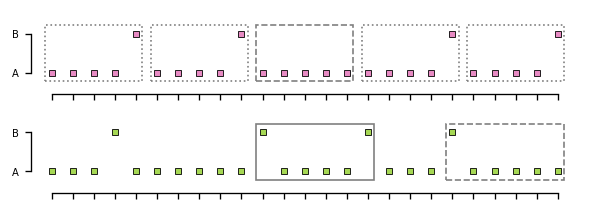
\includegraphics{figures/fig1.png}
\caption{Tones of two different frequencies (A=440 Hz, B=449 Hz) were
presented in two blocked conditions: In the \enquote{predictable}
condition (top half), tones followed a simple pattern in which a single
B-tone followed four A-tones. Some designated B-tones were replaced by
A-tones (\enquote{pattern deviants}). In the \enquote{random} condition
(lower half), tones were presented in a pseudo-random fashion ()}
\end{figure}

Stimuli consisted of pure sinusoidal tones with a duration of 50 ms
(including a 10 ms cosine on/off ramp), presented isochronously at a
stimulation onsets asynchrony (SOA) of 100 ms for study 1 and 150 ms for
study 2. Participants where seated in a electromagnetically shielded and
sound-proofed cabin while administering a total of 40 blocks containing
a mixture of frequent 440 Hz tones (\enquote{A} tones) and infrequent
449 Hz tones (\enquote{B} tones). In one half of the blocks, tones were
presented in pseudo-random order (e.g.~A-A-A-B-A-B-A\}, \enquote{random}
condition), while in the remaining block tone presentation followed a
simple pattern in which a five-tone-sequence of four frequent tones and
one infrequent tone (i.e.~A-A-A-A-B) was repeated cyclically
(\enquote{predictable} condition). The ratio of frequent and infrequent
tones was 10\% for both conditions. Within the predictable condition,
10\% of designated (infrequent) B tones were replaced by A tones,
resulting in sporadic five-tone sequences consisting solely of A tones
(i.e.~A-A-A-A-A), thus violating the predictability rule. To assure
comparability of local histories between tones in both conditions,
randomly arranged tones were interspersed with sequences mimicking
aforementioned patterns from the predictable condition (B-A-A-A-A-B and
B-A-A-A-A-A) in the random condition. A grand total of 2000 tones in
study 1 and 4000 tones in study 2 were delivered to each participant.

\hypertarget{data-acquisition-1}{%
\subsubsection{Data Acquisition}\label{data-acquisition-1}}

Electrophysiological data was recorded from active
silver-silver-chloride (\emph{Ag}-\emph{AgCl}) electrodes using an
ActiveTwo amplifier (BioSemi B.V., Amsterdam, The Netherlands).
Acquisition was monitored online to ensure optimal data quality. A total
of 39 channels were obtained using a 32-electrode-cap and 7 external
electrodes. Scalp electrode locations conformed to the international
10--20 system. Horizontal and vertical eye movement was obtained using
two bipolar configurations with electrodes placed around the lateral
canthi of the eyes and above and below the right eye. Additionally,
electrodes were placed on the tip of the nose and at the left and right
mastoid sites. Data was sampled at 512 Hz and on-line filtered at 1000
Hz.

\hypertarget{analysis-pipeline}{%
\subsection{Analysis Pipeline}\label{analysis-pipeline}}

Data prepossessing was implemented using a custom pipeline based on the
\emph{MNE Python} software package (Gramfort, 2013) using \emph{Python
3.7}. All computations were carried out on a cluster operated by the
University Computation Center of the University of Leipzig. Code used in
thesis is publicly available at
\url{https://github.com/marcpabst/xmas-oddballmatch}.

\hypertarget{bad-channel-detection-and-interpolation}{%
\subsubsection{Bad Channel Detection and
Interpolation}\label{bad-channel-detection-and-interpolation}}

Firstly, EEG data was subject to the ZapLine procedure (de Cheveigné,
2020) to remove line noise contamination. A fivefold detection procedure
as described by Bigdely-Shamlo et al. (2015) was then used to detect and
subsequently interpolate bad channels. This specifically included the
detection of channels thain contain prolonged segments with verry small
values (i.e.~flat channels), the exclusion of channels based on robust
standard deviation (deviation criterion), unusualy pronounced
high-frequency noise (noisiness criterion), and the removal of channels
that were poorly predicted by nearby channels (correlation criterion and
predictability criterion). Channels considered bad by one or more of
these methods were removed and interpolated using spherical splines
(Perrin et al., 1989). Electrode locations for interpolations were
informed by the BESA Spherical Head Model.

\hypertarget{independent-component-analysis}{%
\subsubsection{Independent Component
Analysis}\label{independent-component-analysis}}

Given the \(\frac{1}{f}\) power spectral density of EEG data, the
estimation independent components (ICs) by independent component
analysis (ICA) would be strongly influenced by high-frequency noise that
is ususally considere brain-irrelevant {[}reference{]}. To mitigate this
effect, a 1-Hz-high-pass filter (134th order hamming-windowed FIR) was
applied prior to ICA (Winkler et al., 2015).

To further reduce artifacts, Artifact Subspace Reconstruction (ASR,
Mullen et al., 2015) was used to identify parts of the data with unusual
characteristics (bursts) which were subsequently removed. ICA was then
carried out using the \emph{Picard} algorithm (Ablin et al., 2018, 2017)
on PCA-whitened data. To avoid rank-deficiency when extracting
components from data with one or more interpolated channels, PCA was
also used for dimensionality reduction to obtain full-ranked data.

The EEGLAB (version 2020.0, Delorme \& Makeig, 2004) software package
and the IClabel plugin (version 1.2.6, Pion-Tonachini et al., 2019) were
used to automatically classify estimated components. Only components
clearly classified (i.e.~confidence above 50\%) as resulting from either
eye movement, muscular, or heartbeat activity were zeroed-out in the
mixing matrix before inversely transform ICs.

\hypertarget{filtering}{%
\subsubsection{Filtering}\label{filtering}}

In line with recommendations from Widmann et al. (2015) and de Cheveigné
\& Nelken (2019), a ORDER finite impulse response (FIR) bandpass filter
from 0.1 Hz to 30 Hz was applied in forward direction only (Hamming
window with 0.0194 passband ripple and 53 dB stopband attenuation).

\hypertarget{epoching-and-averaging}{%
\subsubsection{Epoching and Averaging}\label{epoching-and-averaging}}

Continuous data was epoched into 400 ms long segments around stimulus
onsets. This included a 100 ms pre-stimulus interval which was used to
perform baseline correction by subtracting its mean amplitude from each
epoch. The AutoReject software package (Jas et al., 2017) was used to
reject bad epochs. The AutoReject algorithm uses cross-validations and
basyan optimaziation to calculate channel-wise peak-to-peak amplitude
thresholds that minimizes the root mean square error (RMSE) between the
mean (after removing the trials marked as bad) and the median of the
data (including all trials). For epochs where only a small subset of
channels exceeded the critical threshold, bad channels were interpolated
instead of removing the whole epoch.

\hypertarget{statistical-analysis}{%
\subsection{Statistical Analysis}\label{statistical-analysis}}

\hypertarget{standard-repetition-effects}{%
\subsubsection{Standard Repetition
Effects}\label{standard-repetition-effects}}

\hypertarget{mmn}{%
\subsubsection{MMN}\label{mmn}}

The dependent variable for analysing missmatch response was calculated
by averaging amplitudes within a time window of ±25 ms around the
maximum negativity obtained by subtracting the mean ERP timecourse
following the (expected) deviant event from the ERP following the
(expected) standard event. To obtain mean amplitudes, ERPs to 4th
position A tones (A-A-A-\textbf{A}-X, \textbf{boldface} indicates the
tone of interest) and B tones (A-A-A-A-\textbf{B}) were averaged
seperatly for both the \emph{random} and the \emph{predictable}
\emph{condition}. For the \emph{random condition}, only tones that were
part of a sequence mimicking the patterns from the predictable condition
were included.

A three-way analysis of variance for repeated measures with the factors
stimulus onset asynchronoy (100 ms vs.~150 ms stimulus onset
asynchrony), condition (predictabe vs random presenation) and stimulus
type (A tones vs.~B tone).

To further analyse Following the pre-registration, a two-way analysis of
variance for repeated measures to test for significant differences of
mean amplitudes in the MMN window between standard and deviant tones
(stimulus type) depending on the condition (predictable vs.~random) was
calculated seperatly for both 100 ms and 150 ms presentation. In line
with Sussman \& Gumenyuk (2005), FZ, F3, F4, FC1, and FC2 electrode
locations were averaged. Greenhouse-Geisser correction for lack of
sphericity was applied when appropriate.

For post-hock comparison, two-tailed Student's t-test were calculated
for . P-values were corrected for multiple comparisons by using the
Benjamini-Hochberg procedure.

\hypertarget{results}{%
\section{Results}\label{results}}

Grand averages of the fronto-cluster (pooled FZ, F3, F4, FC1, and FC2
electrode locations) of event-related potentials for A tones
(A-A-A-\textbf{A}-X) and B tones (A-A-A-A-\textbf{B}) and their
difference (B-ERP - A-ERP) are displayed in figure 2 for both 100 ms
(left panel) and 150 ms (right panel) stimulus onset asynchrony. The top
half of each panel shows ERPs in the \emph{predictable condition} while
the lower halfs depicts ERPs in the \emph{random condition}. For both
presentation rates, clear rythms matching the presentation frequency of
10 Hz (100 ms) respectivly 6.667 Hz (150 ms) are seen resulting from
overlap of neighboring tones. Panels also show the distribution of
amplitude differences in the MMN latency window as defined above (110 ms
to 160 ms after stimulus onset) across particpants and the difference of
topographic maps averaged over the same interval.

Figure 3 display

\begin{figure}
\centering
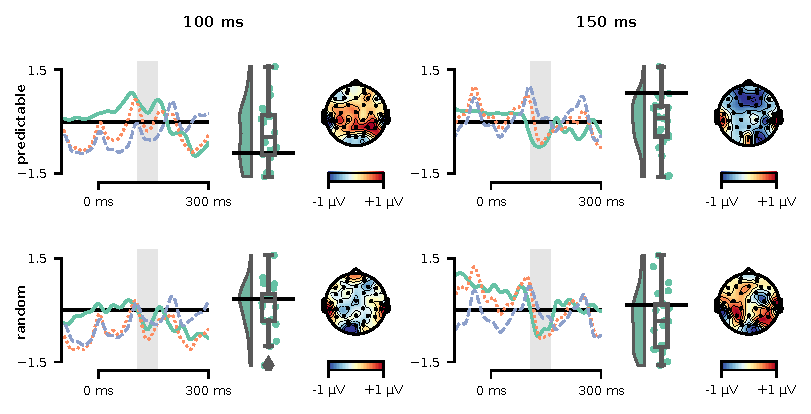
\includegraphics{figures/fig2.pdf}
\caption{ERP grand averages (pooled FZ, F3, F4, FC1, and FC2 electrode
locations) for an SOA of 100 ms (left) and 150 ms (right), for A tones
(A-A-A-\textbf{A}-X, blue dashed lines) and B tones (A-A-A-A-\textbf{B},
orange dashed line) and their difference (B - A, green solid line).
Upper panels show ERPs for tones presented in a predcitable pattern
(\emph{predcitable condition}) while lower panels show ERPs for tones
presented in pseudo-random order (\emph{random condition}). Shaded area
marks MMN latency window (110 ms to 160 ms) used to calculate the
distribution of amplitude differences across particpants (middle of each
panel) and the difference of topographic maps averaged over the same
interval (right of each panel).}
\end{figure}

\begin{figure}
\centering
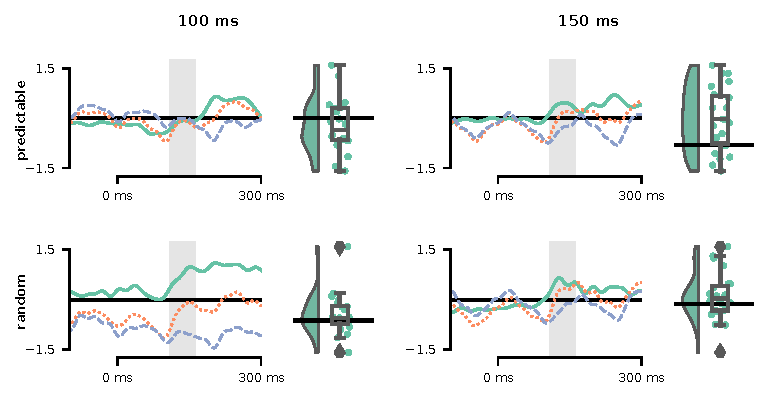
\includegraphics{figures/fig4.pdf}
\caption{ERP grand averages (pooled M1, M2 electrode locations) for an
SOA of 100 ms (left) and 150 ms (right), for A tones
(A-A-A-\textbf{A}-X, blue dashed lines) and B tones (A-A-A-A-\textbf{B},
orange dashed line) and their difference (B - A, green solid line).
Upper panels show ERPs for tones presented in a predcitable pattern
(\emph{predcitable condition}) while lower panels show ERPs for tones
presented in pseudo-random order (\emph{random condition}). Shaded area
marks MMN latency window (110 ms to 160 ms) used to calculate the
distribution of amplitude differences across particpants.}
\end{figure}

\begin{figure}
\centering
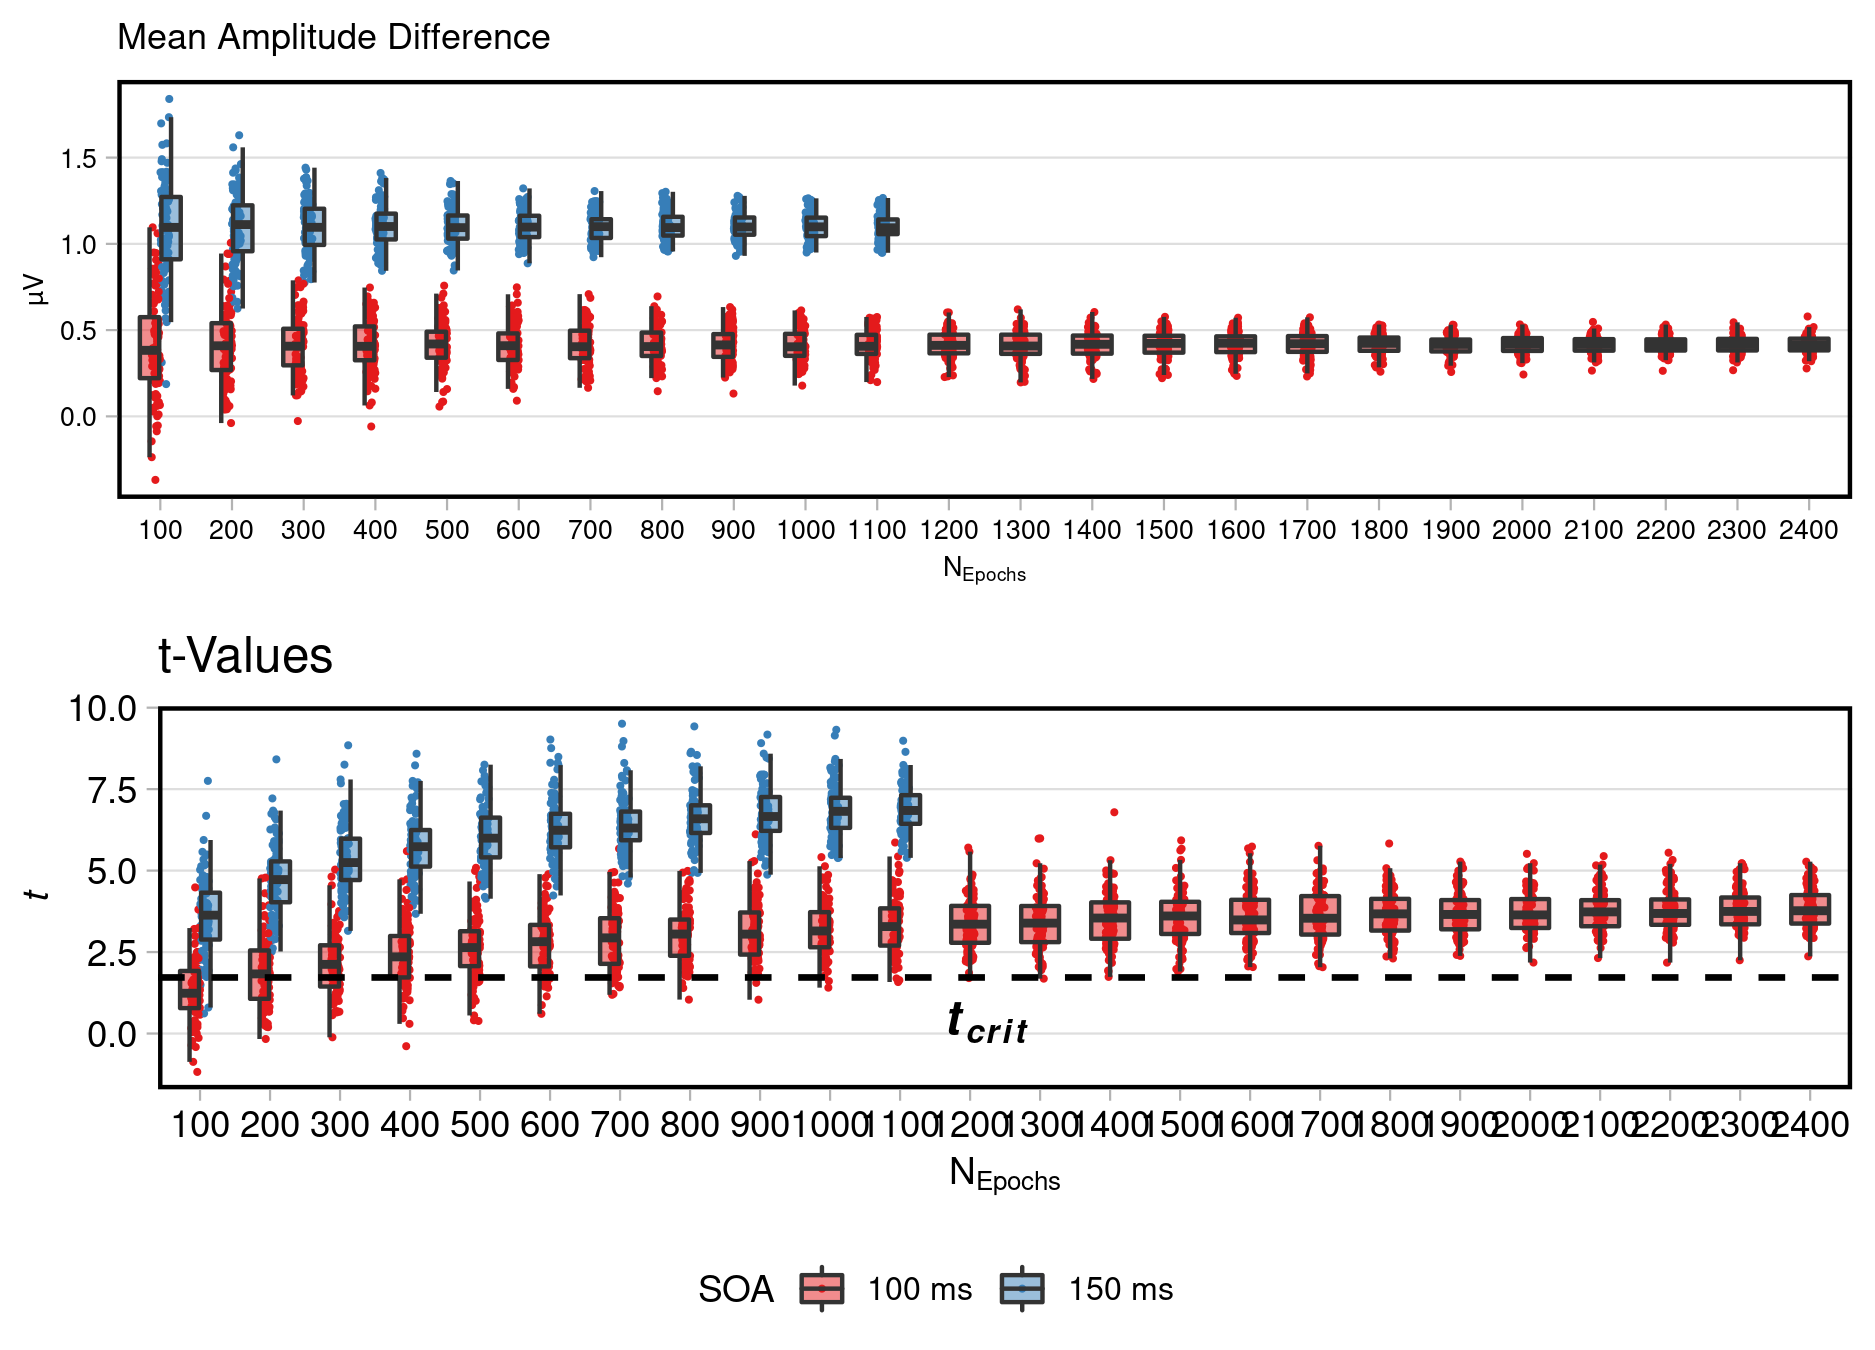
\includegraphics{figures/fig3.png}
\caption{Cadption!!!}
\end{figure}

For the 100 ms stimulation rate, the three-way ANOVA yielded a
significant main effect for stimulus type (\(F(1,19) = 5.00\),
\(p = 0.0380\)) but not for condition (\(F(1,19) = 0.73\),
\(p = 0.4040\)). As expected, a main effect for electrode was found,
indicating that pooled mastoids and the pooled frontal electrodes
differed significantly (\(F(1,19) = 9.68\), \(p = 0.0060\)). While there
was no effect for the two-way interaction \emph{stimulus type x
condition} (\(F(1,19) = 0.58\), \(p = 0.4540\)), their three-way
interaction including the \emph{electrode} term was significant
(\(F(1,19) = 11.44\), \(p = 0.0030\)).

For the 150 ms stimulation rate, the three-way ANOVA yielded a
significant main effect for stimulus type (\(F(1,22) = 9.33\),
\(p = 0.0060\)) but not for condition (\(F(1,22) = 2.40\),
\(p = 0.1360\)). As expected, a main effect for electrode was found,
indicating that pooled mastoids and the pooled frontal electrodes
differed significantly (\(F(1,22) = 10.26\), \(p = 0.0040\)). While
there was no effect for the two-way interaction \emph{stimulus type x
condition} (\(F(1,22) = 0.02\), \(p = 0.8780\)), their three-way
interaction including the \emph{electrode} term was significant
(\(F(1,22) = 6.92\), \(p = 0.0150\)).

For the 150 ms stimulation rate, the 2-way ANOVA yielded a significant
main effect for stimulus type (\(F(1,22) = 56.54\), \(p = 0.0000\)) but
not for condition (\(F(1,22) = 4.80\), \(p = 0.0390\)) or stimulus type
x condition interaction (\(F(1,22) = 4.20\), \(p = 0.0530\)). In
contrast, when presenting tones with a stimulus-onset-assychrnony of 100
ms, no such effects were found for the factor condition
(\(F(1,22) = 4.80\), \(p = 0.0390\)), stimulus type
(\(F(1,22) = 56.54\), \(p = 0.0000\)), or interaction
(\(F(1,22) = 4.20\), \(p = 0.0530\)).


  \providecommand{\huxb}[2]{\arrayrulecolor[RGB]{#1}\global\arrayrulewidth=#2pt}
  \providecommand{\huxvb}[2]{\color[RGB]{#1}\vrule width #2pt}
  \providecommand{\huxtpad}[1]{\rule{0pt}{#1}}
  \providecommand{\huxbpad}[1]{\rule[-#1]{0pt}{#1}}

\begin{table}[ht]
\begin{centerbox}
\begin{threeparttable}
\captionsetup{justification=centering,singlelinecheck=off}
\caption{Results of the 3-way ANOVA (condition x stimulus x electrode) for repeated measures conducted on the mean ERP-amplitudes (time window 111 - 161 ms) at electrode Fz (upper section). The significant interaction between the three factors included was further analyzed by 2-way ANOVAS (stimulus x electrode) conducted separately for the random condition (middle section) and the predictable condition (lower section).}
 \setlength{\tabcolsep}{0pt}
\begin{tabular}{l l l l l l l l}


\hhline{>{\huxb{0, 0, 0}{0.4}}->{\huxb{0, 0, 0}{0.4}}->{\huxb{0, 0, 0}{0.4}}->{\huxb{0, 0, 0}{0.4}}->{\huxb{0, 0, 0}{0.4}}->{\huxb{0, 0, 0}{0.4}}->{\huxb{0, 0, 0}{0.4}}->{\huxb{0, 0, 0}{0.4}}-}
\arrayrulecolor{black}

\multicolumn{1}{!{\huxvb{0, 0, 0}{0}}l!{\huxvb{0, 0, 0}{0}}}{\huxtpad{6pt + 1em}\raggedright \hspace{0pt} \rotatebox{90}{\textbf{}} \hspace{6pt}\huxbpad{6pt}} &
\multicolumn{1}{l!{\huxvb{0, 0, 0}{0}}}{\huxtpad{6pt + 1em}\raggedright \hspace{6pt} \textbf{Effect} \hspace{6pt}\huxbpad{6pt}} &
\multicolumn{1}{r!{\huxvb{0, 0, 0}{0}}}{\huxtpad{6pt + 1em}\raggedleft \hspace{6pt} \textbf{DFn} \hspace{6pt}\huxbpad{6pt}} &
\multicolumn{1}{r!{\huxvb{0, 0, 0}{0}}}{\huxtpad{6pt + 1em}\raggedleft \hspace{6pt} \textbf{DFd} \hspace{6pt}\huxbpad{6pt}} &
\multicolumn{1}{r!{\huxvb{0, 0, 0}{0}}}{\huxtpad{6pt + 1em}\raggedleft \hspace{6pt} \textbf{F} \hspace{6pt}\huxbpad{6pt}} &
\multicolumn{1}{r!{\huxvb{0, 0, 0}{0}}}{\huxtpad{6pt + 1em}\raggedleft \hspace{6pt} \textbf{p} \hspace{6pt}\huxbpad{6pt}} &
\multicolumn{1}{l!{\huxvb{0, 0, 0}{0}}}{\huxtpad{6pt + 1em}\raggedright \hspace{6pt} \textbf{p$<$.05} \hspace{6pt}\huxbpad{6pt}} &
\multicolumn{1}{r!{\huxvb{0, 0, 0}{0}}}{\huxtpad{6pt + 1em}\raggedleft \hspace{6pt} \textbf{ges} \hspace{0pt}\huxbpad{6pt}} \tabularnewline[-0.5pt]


\hhline{>{\huxb{0, 0, 0}{0.4}}->{\huxb{0, 0, 0}{0.4}}->{\huxb{0, 0, 0}{0.4}}->{\huxb{0, 0, 0}{0.4}}->{\huxb{0, 0, 0}{0.4}}->{\huxb{0, 0, 0}{0.4}}->{\huxb{0, 0, 0}{0.4}}->{\huxb{0, 0, 0}{0.4}}-}
\arrayrulecolor{black}

\multicolumn{1}{!{\huxvb{0, 0, 0}{0}}l!{\huxvb{0, 0, 0}{0}}}{} &
\multicolumn{1}{l!{\huxvb{0, 0, 0}{0}}}{\huxtpad{6pt + 1em}\raggedright \hspace{6pt} Condition \hspace{6pt}\huxbpad{6pt}} &
\multicolumn{1}{r!{\huxvb{0, 0, 0}{0}}}{\huxtpad{6pt + 1em}\raggedleft \hspace{6pt} 1 \hspace{6pt}\huxbpad{6pt}} &
\multicolumn{1}{r!{\huxvb{0, 0, 0}{0}}}{\huxtpad{6pt + 1em}\raggedleft \hspace{6pt} 19 \hspace{6pt}\huxbpad{6pt}} &
\multicolumn{1}{r!{\huxvb{0, 0, 0}{0}}}{\huxtpad{6pt + 1em}\raggedleft \hspace{6pt} 0.831 \hspace{6pt}\huxbpad{6pt}} &
\multicolumn{1}{r!{\huxvb{0, 0, 0}{0}}}{\huxtpad{6pt + 1em}\raggedleft \hspace{6pt} 0.373~~~ \hspace{6pt}\huxbpad{6pt}} &
\multicolumn{1}{l!{\huxvb{0, 0, 0}{0}}}{\huxtpad{6pt + 1em}\raggedright \hspace{6pt}  \hspace{6pt}\huxbpad{6pt}} &
\multicolumn{1}{r!{\huxvb{0, 0, 0}{0}}}{\huxtpad{6pt + 1em}\raggedleft \hspace{6pt} 0.008~~~ \hspace{0pt}\huxbpad{6pt}} \tabularnewline[-0.5pt]


\hhline{}
\arrayrulecolor{black}

\multicolumn{1}{!{\huxvb{0, 0, 0}{0}}l!{\huxvb{0, 0, 0}{0}}}{} &
\multicolumn{1}{l!{\huxvb{0, 0, 0}{0}}}{\huxtpad{6pt + 1em}\raggedright \hspace{6pt} StimulusType \hspace{6pt}\huxbpad{6pt}} &
\multicolumn{1}{r!{\huxvb{0, 0, 0}{0}}}{\huxtpad{6pt + 1em}\raggedleft \hspace{6pt} 1 \hspace{6pt}\huxbpad{6pt}} &
\multicolumn{1}{r!{\huxvb{0, 0, 0}{0}}}{\huxtpad{6pt + 1em}\raggedleft \hspace{6pt} 19 \hspace{6pt}\huxbpad{6pt}} &
\multicolumn{1}{r!{\huxvb{0, 0, 0}{0}}}{\huxtpad{6pt + 1em}\raggedleft \hspace{6pt} 1.05~ \hspace{6pt}\huxbpad{6pt}} &
\multicolumn{1}{r!{\huxvb{0, 0, 0}{0}}}{\huxtpad{6pt + 1em}\raggedleft \hspace{6pt} 0.318~~~ \hspace{6pt}\huxbpad{6pt}} &
\multicolumn{1}{l!{\huxvb{0, 0, 0}{0}}}{\huxtpad{6pt + 1em}\raggedright \hspace{6pt}  \hspace{6pt}\huxbpad{6pt}} &
\multicolumn{1}{r!{\huxvb{0, 0, 0}{0}}}{\huxtpad{6pt + 1em}\raggedleft \hspace{6pt} 0.002~~~ \hspace{0pt}\huxbpad{6pt}} \tabularnewline[-0.5pt]


\hhline{}
\arrayrulecolor{black}

\multicolumn{1}{!{\huxvb{0, 0, 0}{0}}l!{\huxvb{0, 0, 0}{0}}}{} &
\multicolumn{1}{l!{\huxvb{0, 0, 0}{0}}}{\huxtpad{6pt + 1em}\raggedright \hspace{6pt} Electrode \hspace{6pt}\huxbpad{6pt}} &
\multicolumn{1}{r!{\huxvb{0, 0, 0}{0}}}{\huxtpad{6pt + 1em}\raggedleft \hspace{6pt} 1 \hspace{6pt}\huxbpad{6pt}} &
\multicolumn{1}{r!{\huxvb{0, 0, 0}{0}}}{\huxtpad{6pt + 1em}\raggedleft \hspace{6pt} 19 \hspace{6pt}\huxbpad{6pt}} &
\multicolumn{1}{r!{\huxvb{0, 0, 0}{0}}}{\huxtpad{6pt + 1em}\raggedleft \hspace{6pt} 0.036 \hspace{6pt}\huxbpad{6pt}} &
\multicolumn{1}{r!{\huxvb{0, 0, 0}{0}}}{\huxtpad{6pt + 1em}\raggedleft \hspace{6pt} 0.852~~~ \hspace{6pt}\huxbpad{6pt}} &
\multicolumn{1}{l!{\huxvb{0, 0, 0}{0}}}{\huxtpad{6pt + 1em}\raggedright \hspace{6pt}  \hspace{6pt}\huxbpad{6pt}} &
\multicolumn{1}{r!{\huxvb{0, 0, 0}{0}}}{\huxtpad{6pt + 1em}\raggedleft \hspace{6pt} 0.000331 \hspace{0pt}\huxbpad{6pt}} \tabularnewline[-0.5pt]


\hhline{}
\arrayrulecolor{black}

\multicolumn{1}{!{\huxvb{0, 0, 0}{0}}l!{\huxvb{0, 0, 0}{0}}}{} &
\multicolumn{1}{l!{\huxvb{0, 0, 0}{0}}}{\huxtpad{6pt + 1em}\raggedright \hspace{6pt} Condition x StimulusType \hspace{6pt}\huxbpad{6pt}} &
\multicolumn{1}{r!{\huxvb{0, 0, 0}{0}}}{\huxtpad{6pt + 1em}\raggedleft \hspace{6pt} 1 \hspace{6pt}\huxbpad{6pt}} &
\multicolumn{1}{r!{\huxvb{0, 0, 0}{0}}}{\huxtpad{6pt + 1em}\raggedleft \hspace{6pt} 19 \hspace{6pt}\huxbpad{6pt}} &
\multicolumn{1}{r!{\huxvb{0, 0, 0}{0}}}{\huxtpad{6pt + 1em}\raggedleft \hspace{6pt} 0.051 \hspace{6pt}\huxbpad{6pt}} &
\multicolumn{1}{r!{\huxvb{0, 0, 0}{0}}}{\huxtpad{6pt + 1em}\raggedleft \hspace{6pt} 0.823~~~ \hspace{6pt}\huxbpad{6pt}} &
\multicolumn{1}{l!{\huxvb{0, 0, 0}{0}}}{\huxtpad{6pt + 1em}\raggedright \hspace{6pt}  \hspace{6pt}\huxbpad{6pt}} &
\multicolumn{1}{r!{\huxvb{0, 0, 0}{0}}}{\huxtpad{6pt + 1em}\raggedleft \hspace{6pt} 7.55e-05 \hspace{0pt}\huxbpad{6pt}} \tabularnewline[-0.5pt]


\hhline{}
\arrayrulecolor{black}

\multicolumn{1}{!{\huxvb{0, 0, 0}{0}}l!{\huxvb{0, 0, 0}{0}}}{} &
\multicolumn{1}{l!{\huxvb{0, 0, 0}{0}}}{\huxtpad{6pt + 1em}\raggedright \hspace{6pt} Condition x Electrode \hspace{6pt}\huxbpad{6pt}} &
\multicolumn{1}{r!{\huxvb{0, 0, 0}{0}}}{\huxtpad{6pt + 1em}\raggedleft \hspace{6pt} 1 \hspace{6pt}\huxbpad{6pt}} &
\multicolumn{1}{r!{\huxvb{0, 0, 0}{0}}}{\huxtpad{6pt + 1em}\raggedleft \hspace{6pt} 19 \hspace{6pt}\huxbpad{6pt}} &
\multicolumn{1}{r!{\huxvb{0, 0, 0}{0}}}{\huxtpad{6pt + 1em}\raggedleft \hspace{6pt} 0.763 \hspace{6pt}\huxbpad{6pt}} &
\multicolumn{1}{r!{\huxvb{0, 0, 0}{0}}}{\huxtpad{6pt + 1em}\raggedleft \hspace{6pt} 0.393~~~ \hspace{6pt}\huxbpad{6pt}} &
\multicolumn{1}{l!{\huxvb{0, 0, 0}{0}}}{\huxtpad{6pt + 1em}\raggedright \hspace{6pt}  \hspace{6pt}\huxbpad{6pt}} &
\multicolumn{1}{r!{\huxvb{0, 0, 0}{0}}}{\huxtpad{6pt + 1em}\raggedleft \hspace{6pt} 0.002~~~ \hspace{0pt}\huxbpad{6pt}} \tabularnewline[-0.5pt]


\hhline{}
\arrayrulecolor{black}

\multicolumn{1}{!{\huxvb{0, 0, 0}{0}}l!{\huxvb{0, 0, 0}{0}}}{} &
\multicolumn{1}{l!{\huxvb{0, 0, 0}{0}}}{\huxtpad{6pt + 1em}\raggedright \hspace{6pt} StimulusType x Electrode \hspace{6pt}\huxbpad{6pt}} &
\multicolumn{1}{r!{\huxvb{0, 0, 0}{0}}}{\huxtpad{6pt + 1em}\raggedleft \hspace{6pt} 1 \hspace{6pt}\huxbpad{6pt}} &
\multicolumn{1}{r!{\huxvb{0, 0, 0}{0}}}{\huxtpad{6pt + 1em}\raggedleft \hspace{6pt} 19 \hspace{6pt}\huxbpad{6pt}} &
\multicolumn{1}{r!{\huxvb{0, 0, 0}{0}}}{\huxtpad{6pt + 1em}\raggedleft \hspace{6pt} 0.797 \hspace{6pt}\huxbpad{6pt}} &
\multicolumn{1}{r!{\huxvb{0, 0, 0}{0}}}{\huxtpad{6pt + 1em}\raggedleft \hspace{6pt} 0.383~~~ \hspace{6pt}\huxbpad{6pt}} &
\multicolumn{1}{l!{\huxvb{0, 0, 0}{0}}}{\huxtpad{6pt + 1em}\raggedright \hspace{6pt}  \hspace{6pt}\huxbpad{6pt}} &
\multicolumn{1}{r!{\huxvb{0, 0, 0}{0}}}{\huxtpad{6pt + 1em}\raggedleft \hspace{6pt} 0.001~~~ \hspace{0pt}\huxbpad{6pt}} \tabularnewline[-0.5pt]


\hhline{}
\arrayrulecolor{black}

\multicolumn{1}{!{\huxvb{0, 0, 0}{0}}l!{\huxvb{0, 0, 0}{0}}}{\multirow[c]{-7}{*}[0ex]{\huxtpad{6pt + 1em}\raggedright \hspace{0pt} \rotatebox{90}{100 ms} \hspace{6pt}\huxbpad{6pt}}} &
\multicolumn{1}{l!{\huxvb{0, 0, 0}{0}}}{\huxtpad{6pt + 1em}\raggedright \hspace{6pt} Condition x StimulusType x Electrode \hspace{6pt}\huxbpad{15pt}} &
\multicolumn{1}{r!{\huxvb{0, 0, 0}{0}}}{\huxtpad{6pt + 1em}\raggedleft \hspace{6pt} 1 \hspace{6pt}\huxbpad{15pt}} &
\multicolumn{1}{r!{\huxvb{0, 0, 0}{0}}}{\huxtpad{6pt + 1em}\raggedleft \hspace{6pt} 19 \hspace{6pt}\huxbpad{15pt}} &
\multicolumn{1}{r!{\huxvb{0, 0, 0}{0}}}{\huxtpad{6pt + 1em}\raggedleft \hspace{6pt} 7.53~ \hspace{6pt}\huxbpad{15pt}} &
\multicolumn{1}{r!{\huxvb{0, 0, 0}{0}}}{\huxtpad{6pt + 1em}\raggedleft \hspace{6pt} 0.013~~~ \hspace{6pt}\huxbpad{15pt}} &
\multicolumn{1}{l!{\huxvb{0, 0, 0}{0}}}{\huxtpad{6pt + 1em}\raggedright \hspace{6pt} * \hspace{6pt}\huxbpad{15pt}} &
\multicolumn{1}{r!{\huxvb{0, 0, 0}{0}}}{\huxtpad{6pt + 1em}\raggedleft \hspace{6pt} 0.01~~~~ \hspace{0pt}\huxbpad{15pt}} \tabularnewline[-0.5pt]


\hhline{}
\arrayrulecolor{black}

\multicolumn{1}{!{\huxvb{0, 0, 0}{0}}l!{\huxvb{0, 0, 0}{0}}}{} &
\multicolumn{1}{l!{\huxvb{0, 0, 0}{0}}}{\huxtpad{15pt + 1em}\raggedright \hspace{6pt} Condition \hspace{6pt}\huxbpad{6pt}} &
\multicolumn{1}{r!{\huxvb{0, 0, 0}{0}}}{\huxtpad{15pt + 1em}\raggedleft \hspace{6pt} 1 \hspace{6pt}\huxbpad{6pt}} &
\multicolumn{1}{r!{\huxvb{0, 0, 0}{0}}}{\huxtpad{15pt + 1em}\raggedleft \hspace{6pt} 22 \hspace{6pt}\huxbpad{6pt}} &
\multicolumn{1}{r!{\huxvb{0, 0, 0}{0}}}{\huxtpad{15pt + 1em}\raggedleft \hspace{6pt} 0.08~ \hspace{6pt}\huxbpad{6pt}} &
\multicolumn{1}{r!{\huxvb{0, 0, 0}{0}}}{\huxtpad{15pt + 1em}\raggedleft \hspace{6pt} 0.78~~~~ \hspace{6pt}\huxbpad{6pt}} &
\multicolumn{1}{l!{\huxvb{0, 0, 0}{0}}}{\huxtpad{15pt + 1em}\raggedright \hspace{6pt}  \hspace{6pt}\huxbpad{6pt}} &
\multicolumn{1}{r!{\huxvb{0, 0, 0}{0}}}{\huxtpad{15pt + 1em}\raggedleft \hspace{6pt} 0.000263 \hspace{0pt}\huxbpad{6pt}} \tabularnewline[-0.5pt]


\hhline{}
\arrayrulecolor{black}

\multicolumn{1}{!{\huxvb{0, 0, 0}{0}}l!{\huxvb{0, 0, 0}{0}}}{} &
\multicolumn{1}{l!{\huxvb{0, 0, 0}{0}}}{\huxtpad{6pt + 1em}\raggedright \hspace{6pt} StimulusType \hspace{6pt}\huxbpad{6pt}} &
\multicolumn{1}{r!{\huxvb{0, 0, 0}{0}}}{\huxtpad{6pt + 1em}\raggedleft \hspace{6pt} 1 \hspace{6pt}\huxbpad{6pt}} &
\multicolumn{1}{r!{\huxvb{0, 0, 0}{0}}}{\huxtpad{6pt + 1em}\raggedleft \hspace{6pt} 22 \hspace{6pt}\huxbpad{6pt}} &
\multicolumn{1}{r!{\huxvb{0, 0, 0}{0}}}{\huxtpad{6pt + 1em}\raggedleft \hspace{6pt} 0.317 \hspace{6pt}\huxbpad{6pt}} &
\multicolumn{1}{r!{\huxvb{0, 0, 0}{0}}}{\huxtpad{6pt + 1em}\raggedleft \hspace{6pt} 0.579~~~ \hspace{6pt}\huxbpad{6pt}} &
\multicolumn{1}{l!{\huxvb{0, 0, 0}{0}}}{\huxtpad{6pt + 1em}\raggedright \hspace{6pt}  \hspace{6pt}\huxbpad{6pt}} &
\multicolumn{1}{r!{\huxvb{0, 0, 0}{0}}}{\huxtpad{6pt + 1em}\raggedleft \hspace{6pt} 0.000339 \hspace{0pt}\huxbpad{6pt}} \tabularnewline[-0.5pt]


\hhline{}
\arrayrulecolor{black}

\multicolumn{1}{!{\huxvb{0, 0, 0}{0}}l!{\huxvb{0, 0, 0}{0}}}{} &
\multicolumn{1}{l!{\huxvb{0, 0, 0}{0}}}{\huxtpad{6pt + 1em}\raggedright \hspace{6pt} Electrode \hspace{6pt}\huxbpad{6pt}} &
\multicolumn{1}{r!{\huxvb{0, 0, 0}{0}}}{\huxtpad{6pt + 1em}\raggedleft \hspace{6pt} 1 \hspace{6pt}\huxbpad{6pt}} &
\multicolumn{1}{r!{\huxvb{0, 0, 0}{0}}}{\huxtpad{6pt + 1em}\raggedleft \hspace{6pt} 22 \hspace{6pt}\huxbpad{6pt}} &
\multicolumn{1}{r!{\huxvb{0, 0, 0}{0}}}{\huxtpad{6pt + 1em}\raggedleft \hspace{6pt} 0.035 \hspace{6pt}\huxbpad{6pt}} &
\multicolumn{1}{r!{\huxvb{0, 0, 0}{0}}}{\huxtpad{6pt + 1em}\raggedleft \hspace{6pt} 0.854~~~ \hspace{6pt}\huxbpad{6pt}} &
\multicolumn{1}{l!{\huxvb{0, 0, 0}{0}}}{\huxtpad{6pt + 1em}\raggedright \hspace{6pt}  \hspace{6pt}\huxbpad{6pt}} &
\multicolumn{1}{r!{\huxvb{0, 0, 0}{0}}}{\huxtpad{6pt + 1em}\raggedleft \hspace{6pt} 0.000301 \hspace{0pt}\huxbpad{6pt}} \tabularnewline[-0.5pt]


\hhline{}
\arrayrulecolor{black}

\multicolumn{1}{!{\huxvb{0, 0, 0}{0}}l!{\huxvb{0, 0, 0}{0}}}{} &
\multicolumn{1}{l!{\huxvb{0, 0, 0}{0}}}{\huxtpad{6pt + 1em}\raggedright \hspace{6pt} Condition x StimulusType \hspace{6pt}\huxbpad{6pt}} &
\multicolumn{1}{r!{\huxvb{0, 0, 0}{0}}}{\huxtpad{6pt + 1em}\raggedleft \hspace{6pt} 1 \hspace{6pt}\huxbpad{6pt}} &
\multicolumn{1}{r!{\huxvb{0, 0, 0}{0}}}{\huxtpad{6pt + 1em}\raggedleft \hspace{6pt} 22 \hspace{6pt}\huxbpad{6pt}} &
\multicolumn{1}{r!{\huxvb{0, 0, 0}{0}}}{\huxtpad{6pt + 1em}\raggedleft \hspace{6pt} 0.16~ \hspace{6pt}\huxbpad{6pt}} &
\multicolumn{1}{r!{\huxvb{0, 0, 0}{0}}}{\huxtpad{6pt + 1em}\raggedleft \hspace{6pt} 0.693~~~ \hspace{6pt}\huxbpad{6pt}} &
\multicolumn{1}{l!{\huxvb{0, 0, 0}{0}}}{\huxtpad{6pt + 1em}\raggedright \hspace{6pt}  \hspace{6pt}\huxbpad{6pt}} &
\multicolumn{1}{r!{\huxvb{0, 0, 0}{0}}}{\huxtpad{6pt + 1em}\raggedleft \hspace{6pt} 0.000124 \hspace{0pt}\huxbpad{6pt}} \tabularnewline[-0.5pt]


\hhline{}
\arrayrulecolor{black}

\multicolumn{1}{!{\huxvb{0, 0, 0}{0}}l!{\huxvb{0, 0, 0}{0}}}{} &
\multicolumn{1}{l!{\huxvb{0, 0, 0}{0}}}{\huxtpad{6pt + 1em}\raggedright \hspace{6pt} Condition x Electrode \hspace{6pt}\huxbpad{6pt}} &
\multicolumn{1}{r!{\huxvb{0, 0, 0}{0}}}{\huxtpad{6pt + 1em}\raggedleft \hspace{6pt} 1 \hspace{6pt}\huxbpad{6pt}} &
\multicolumn{1}{r!{\huxvb{0, 0, 0}{0}}}{\huxtpad{6pt + 1em}\raggedleft \hspace{6pt} 22 \hspace{6pt}\huxbpad{6pt}} &
\multicolumn{1}{r!{\huxvb{0, 0, 0}{0}}}{\huxtpad{6pt + 1em}\raggedleft \hspace{6pt} 1.13~ \hspace{6pt}\huxbpad{6pt}} &
\multicolumn{1}{r!{\huxvb{0, 0, 0}{0}}}{\huxtpad{6pt + 1em}\raggedleft \hspace{6pt} 0.299~~~ \hspace{6pt}\huxbpad{6pt}} &
\multicolumn{1}{l!{\huxvb{0, 0, 0}{0}}}{\huxtpad{6pt + 1em}\raggedright \hspace{6pt}  \hspace{6pt}\huxbpad{6pt}} &
\multicolumn{1}{r!{\huxvb{0, 0, 0}{0}}}{\huxtpad{6pt + 1em}\raggedleft \hspace{6pt} 0.003~~~ \hspace{0pt}\huxbpad{6pt}} \tabularnewline[-0.5pt]


\hhline{}
\arrayrulecolor{black}

\multicolumn{1}{!{\huxvb{0, 0, 0}{0}}l!{\huxvb{0, 0, 0}{0}}}{} &
\multicolumn{1}{l!{\huxvb{0, 0, 0}{0}}}{\huxtpad{6pt + 1em}\raggedright \hspace{6pt} StimulusType x Electrode \hspace{6pt}\huxbpad{6pt}} &
\multicolumn{1}{r!{\huxvb{0, 0, 0}{0}}}{\huxtpad{6pt + 1em}\raggedleft \hspace{6pt} 1 \hspace{6pt}\huxbpad{6pt}} &
\multicolumn{1}{r!{\huxvb{0, 0, 0}{0}}}{\huxtpad{6pt + 1em}\raggedleft \hspace{6pt} 22 \hspace{6pt}\huxbpad{6pt}} &
\multicolumn{1}{r!{\huxvb{0, 0, 0}{0}}}{\huxtpad{6pt + 1em}\raggedleft \hspace{6pt} 20.8~~ \hspace{6pt}\huxbpad{6pt}} &
\multicolumn{1}{r!{\huxvb{0, 0, 0}{0}}}{\huxtpad{6pt + 1em}\raggedleft \hspace{6pt} 0.000155 \hspace{6pt}\huxbpad{6pt}} &
\multicolumn{1}{l!{\huxvb{0, 0, 0}{0}}}{\huxtpad{6pt + 1em}\raggedright \hspace{6pt} * \hspace{6pt}\huxbpad{6pt}} &
\multicolumn{1}{r!{\huxvb{0, 0, 0}{0}}}{\huxtpad{6pt + 1em}\raggedleft \hspace{6pt} 0.026~~~ \hspace{0pt}\huxbpad{6pt}} \tabularnewline[-0.5pt]


\hhline{}
\arrayrulecolor{black}

\multicolumn{1}{!{\huxvb{0, 0, 0}{0}}l!{\huxvb{0, 0, 0}{0}}}{\multirow[c]{-7}{*}[0ex]{\huxtpad{15pt + 1em}\raggedright \hspace{0pt} \rotatebox{90}{150 ms} \hspace{6pt}\huxbpad{6pt}}} &
\multicolumn{1}{l!{\huxvb{0, 0, 0}{0}}}{\huxtpad{6pt + 1em}\raggedright \hspace{6pt} Condition x StimulusType x Electrode \hspace{6pt}\huxbpad{6pt}} &
\multicolumn{1}{r!{\huxvb{0, 0, 0}{0}}}{\huxtpad{6pt + 1em}\raggedleft \hspace{6pt} 1 \hspace{6pt}\huxbpad{6pt}} &
\multicolumn{1}{r!{\huxvb{0, 0, 0}{0}}}{\huxtpad{6pt + 1em}\raggedleft \hspace{6pt} 22 \hspace{6pt}\huxbpad{6pt}} &
\multicolumn{1}{r!{\huxvb{0, 0, 0}{0}}}{\huxtpad{6pt + 1em}\raggedleft \hspace{6pt} 0.053 \hspace{6pt}\huxbpad{6pt}} &
\multicolumn{1}{r!{\huxvb{0, 0, 0}{0}}}{\huxtpad{6pt + 1em}\raggedleft \hspace{6pt} 0.819~~~ \hspace{6pt}\huxbpad{6pt}} &
\multicolumn{1}{l!{\huxvb{0, 0, 0}{0}}}{\huxtpad{6pt + 1em}\raggedright \hspace{6pt}  \hspace{6pt}\huxbpad{6pt}} &
\multicolumn{1}{r!{\huxvb{0, 0, 0}{0}}}{\huxtpad{6pt + 1em}\raggedleft \hspace{6pt} 4.63e-05 \hspace{0pt}\huxbpad{6pt}} \tabularnewline[-0.5pt]


\hhline{>{\huxb{0, 0, 0}{0.4}}->{\huxb{0, 0, 0}{0.4}}->{\huxb{0, 0, 0}{0.4}}->{\huxb{0, 0, 0}{0.4}}->{\huxb{0, 0, 0}{0.4}}->{\huxb{0, 0, 0}{0.4}}->{\huxb{0, 0, 0}{0.4}}->{\huxb{0, 0, 0}{0.4}}-}
\arrayrulecolor{black}
\end{tabular}
\end{threeparttable}\par\end{centerbox}

\end{table}



% latex table generated in R 4.0.3 by xtable 1.8-4 package
% Tue Nov 17 13:11:39 2020
\begin{table}[ht]
\centering
\begin{tabulary}{\textwidth}{lrrrrlr}
  \toprule
Effect & DFn & DFd & F & p & p$<$.05 & ges \\ 
  \midrule
Condition & 1.00 & 22.00 & 1.53 & 0.23 &  & 0.01 \\ 
  StimulusType & 1.00 & 22.00 & 0.61 & 0.44 &  & 0.00 \\ 
  Electrode & 4.00 & 88.00 & 9.73 & 0.00 & * & 0.15 \\ 
  Condition x StimulusType & 1.00 & 22.00 & 0.78 & 0.39 &  & 0.00 \\ 
  Condition x Electrode & 4.00 & 88.00 & 2.09 & 0.09 &  & 0.01 \\ 
  StimulusType x Electrode & 4.00 & 88.00 & 43.51 & 0.00 & * & 0.26 \\ 
  Condition x StimulusType x Electrode & 4.00 & 88.00 & 5.15 & 0.00 & * & 0.01 \\ 
   \bottomrule
\end{tabulary}
\end{table}


% latex table generated in R 4.0.3 by xtable 1.8-4 package
% Tue Dec  8 16:48:32 2020
\begin{table}[ht]
\centering
\begin{tabulary}{\textwidth}{lrrrrlr}
  \hline
Effect & DFn & DFd & F & p & p$<$.05 & ges \\ 
  \hline
Condition & 1.00 & 19.00 & 0.85 & 0.37 &  & 0.01 \\ 
  StimulusType & 1.00 & 19.00 & 0.83 & 0.37 &  & 0.00 \\ 
  Electrode & 1.00 & 19.00 & 0.13 & 0.72 &  & 0.00 \\ 
  Condition x StimulusType & 1.00 & 19.00 & 0.03 & 0.86 &  & 0.00 \\ 
  Condition x Electrode & 1.00 & 19.00 & 0.90 & 0.35 &  & 0.00 \\ 
  StimulusType x Electrode & 1.00 & 19.00 & 0.63 & 0.44 &  & 0.00 \\ 
  Condition x StimulusType x Electrode & 1.00 & 19.00 & 7.21 & 0.01 & * & 0.01 \\ 
   \hline
\end{tabulary}
\end{table}


% latex table generated in R 4.0.3 by xtable 1.8-4 package
% Wed Nov 25 17:29:22 2020
\begin{table}[ht]
\centering
\begin{tabulary}{\textwidth}{lrrrrlr}
  \hline
Effect & DFn & DFd & F & p & p$<$.05 & ges \\ 
  \hline
Condition & 1.00 & 19.00 & 0.16 & 0.69 &  & 0.00 \\ 
  StimulusType & 1.00 & 19.00 & 0.01 & 0.94 &  & 0.00 \\ 
  Condition x StimulusType & 1.00 & 19.00 & 16.75 & 0.00 & * & 0.01 \\ 
   \hline
\end{tabulary}
\caption{Results of the 3-way ANOVA (condition x stimulus x electrode) for repeated measures conducted on the mean ERP-amplitudes (time window 111 - 161 ms) at electrode Fz (upper section). The significant interaction between the three factors included was further analyzed by 2-way ANOVAS (stimulus x electrode) conducted separately for the random condition (middle section) and the predictable condition (lower section).} 
\end{table}


% latex table generated in R 4.0.3 by xtable 1.8-4 package
% Tue Nov 17 13:11:38 2020
\begin{table}[ht]
\centering
\begin{tabulary}{\textwidth}{llrrrr}
  \toprule
group1 & group2 & df & t & p & p.adj \\ 
  \midrule
CZ & FZ & 19.00 & -0.57 & 0.57 & 1.00 \\ 
  CZ & M1 & 19.00 & 3.63 & 0.00 & 0.02 \\ 
  CZ & M2 & 19.00 & 3.22 & 0.00 & 0.03 \\ 
  CZ & mastoids\_pooled & 19.00 & 3.52 & 0.00 & 0.02 \\ 
  FZ & M1 & 19.00 & 3.37 & 0.00 & 0.03 \\ 
  FZ & M2 & 19.00 & 3.02 & 0.01 & 0.04 \\ 
  FZ & mastoids\_pooled & 19.00 & 3.27 & 0.00 & 0.03 \\ 
  M1 & M2 & 19.00 & -1.07 & 0.30 & 1.00 \\ 
  M1 & mastoids\_pooled & 19.00 & -1.07 & 0.30 & 1.00 \\ 
  M2 & mastoids\_pooled & 19.00 & 1.07 & 0.30 & 1.00 \\ 
   \bottomrule
\end{tabulary}
\end{table}


% latex table generated in R 4.0.3 by xtable 1.8-4 package
% Wed Nov 25 17:29:23 2020
\begin{table}[ht]
\centering
\begin{tabulary}{\textwidth}{lrrrrlr}
  \hline
Effect & DFn & DFd & F & p & p$<$.05 & ges \\ 
  \hline
Condition & 1.00 & 22.00 & 0.95 & 0.34 &  & 0.01 \\ 
  StimulusType & 1.00 & 22.00 & 22.67 & 0.00 & * & 0.04 \\ 
  Condition x StimulusType & 1.00 & 22.00 & 0.03 & 0.87 &  & 0.00 \\ 
   \hline
\end{tabulary}
\end{table}


% latex table generated in R 4.0.3 by xtable 1.8-4 package
% Tue Nov 17 13:11:39 2020
\begin{table}[ht]
\centering
\begin{tabulary}{\textwidth}{lrrrrlr}
  \toprule
Effect & DFn & DFd & F & p & p$<$.05 & ges \\ 
  \midrule
Condition & 1.00 & 22.00 & 1.53 & 0.23 &  & 0.01 \\ 
  StimulusType & 1.00 & 22.00 & 0.61 & 0.44 &  & 0.00 \\ 
  Electrode & 4.00 & 88.00 & 9.73 & 0.00 & * & 0.15 \\ 
  Condition x StimulusType & 1.00 & 22.00 & 0.78 & 0.39 &  & 0.00 \\ 
  Condition x Electrode & 4.00 & 88.00 & 2.09 & 0.09 &  & 0.01 \\ 
  StimulusType x Electrode & 4.00 & 88.00 & 43.51 & 0.00 & * & 0.26 \\ 
  Condition x StimulusType x Electrode & 4.00 & 88.00 & 5.15 & 0.00 & * & 0.01 \\ 
   \bottomrule
\end{tabulary}
\end{table}


% latex table generated in R 4.0.3 by xtable 1.8-4 package
% Tue Nov 17 13:11:39 2020
\begin{table}[ht]
\centering
\begin{tabulary}{\textwidth}{llrrrr}
  \toprule
group1 & group2 & df & t & p & p.adj \\ 
  \midrule
CZ & FZ & 22.00 & 1.43 & 0.17 & 0.30 \\ 
  CZ & M1 & 22.00 & -2.65 & 0.01 & 0.07 \\ 
  CZ & M2 & 22.00 & -3.59 & 0.00 & 0.01 \\ 
  CZ & mastoids\_pooled & 22.00 & -3.16 & 0.01 & 0.03 \\ 
  FZ & M1 & 22.00 & -2.73 & 0.01 & 0.07 \\ 
  FZ & M2 & 22.00 & -3.63 & 0.00 & 0.01 \\ 
  FZ & mastoids\_pooled & 22.00 & -3.21 & 0.00 & 0.03 \\ 
  M1 & M2 & 22.00 & -1.87 & 0.07 & 0.30 \\ 
  M1 & mastoids\_pooled & 22.00 & -1.87 & 0.07 & 0.30 \\ 
  M2 & mastoids\_pooled & 22.00 & 1.87 & 0.07 & 0.30 \\ 
   \bottomrule
\end{tabulary}
\end{table}


\newpage

\hypertarget{references}{%
\section{References}\label{references}}

MMN explained by positiviy (?) -\textgreater{} first-order MMN?

\hypertarget{refs}{}
\begin{cslreferences}
\leavevmode\hypertarget{ref-ablinFasterIndependentComponent2018}{}%
Ablin, P., Cardoso, J.-F., \& Gramfort, A. (2018). Faster independent
component analysis by preconditioning with Hessian approximations.
\emph{IEEE Transactions on Signal Processing}, \emph{66}(15),
4040--4049. \url{https://doi.org/10.1109/TSP.2018.2844203}

\leavevmode\hypertarget{ref-ablinFasterICAOrthogonal2017}{}%
Ablin, P., Cardoso, J.-F., \& Gramfort, A. (2017). Faster ICA under
orthogonal constraint. \emph{arXiv:1711.10873 {[}Stat{]}}.
\url{http://arxiv.org/abs/1711.10873}

\leavevmode\hypertarget{ref-alainBrainIndicesAutomatic1994}{}%
Alain, C., Woods, D. L., \& Ogawa, K. H. (1994). Brain indices of
automatic pattern processing: \emph{NeuroReport}, \emph{6}(1), 140--144.
\url{https://doi.org/10.1097/00001756-199412300-00036}

\leavevmode\hypertarget{ref-bigdely-shamloPREPPipelineStandardized2015}{}%
Bigdely-Shamlo, N., Mullen, T., Kothe, C., Su, K.-M., \& Robbins, K. A.
(2015). The PREP pipeline: standardized preprocessing for large-scale
EEG analysis. \emph{Frontiers in Neuroinformatics}, \emph{9}.
\url{https://doi.org/10.3389/fninf.2015.00016}

\leavevmode\hypertarget{ref-decheveigneZapLineSimpleEffective2020}{}%
de Cheveigné, A. (2020). ZapLine: A simple and effective method to
remove power line artifacts. \emph{NeuroImage}, \emph{207}, 116356.
\url{https://doi.org/10.1016/j.neuroimage.2019.116356}

\leavevmode\hypertarget{ref-decheveigneFiltersWhenWhy2019}{}%
de Cheveigné, A., \& Nelken, I. (2019). Filters: When, Why, and How
(Not) to Use Them. \emph{Neuron}, \emph{102}(2), 280--293.
\url{https://doi.org/10.1016/j.neuron.2019.02.039}

\leavevmode\hypertarget{ref-delormeEEGLABOpenSource2004}{}%
Delorme, A., \& Makeig, S. (2004). EEGLAB: an open source toolbox for
analysis of single-trial EEG dynamics including independent component
analysis. \emph{Journal of Neuroscience Methods}, \emph{134}(1), 9--21.
\url{https://doi.org/10.1016/j.jneumeth.2003.10.009}

\leavevmode\hypertarget{ref-gramfortMEGEEGData2013}{}%
Gramfort, A. (2013). MEG and EEG data analysis with MNE-Python.
\emph{Frontiers in Neuroscience}, \emph{7}.
\url{https://doi.org/10.3389/fnins.2013.00267}

\leavevmode\hypertarget{ref-heDevelopmentInfantMismatch2009}{}%
He, C., Hotson, L., \& Trainor, L. J. (2009). Development of infant
mismatch responses to auditory pattern changes between 2 and 4 months
old. \emph{European Journal of Neuroscience}, \emph{29}(4), 861--867.
\url{https://doi.org/10.1111/j.1460-9568.2009.06625.x}

\leavevmode\hypertarget{ref-jasAutorejectAutomatedArtifact2017}{}%
Jas, M., Engemann, D. A., Bekhti, Y., Raimondo, F., \& Gramfort, A.
(2017). Autoreject: Automated artifact rejection for MEG and EEG data.
\emph{NeuroImage}, \emph{159}, 417--429.
\url{https://doi.org/10.1016/j.neuroimage.2017.06.030}

\leavevmode\hypertarget{ref-mullenRealtimeNeuroimagingCognitive2015}{}%
Mullen, T. R., Kothe, C. A. E., Chi, Y. M., Ojeda, A., Kerth, T.,
Makeig, S., Jung, T.-P., \& Cauwenberghs, G. (2015). Real-time
neuroimaging and cognitive monitoring using wearable dry EEG. \emph{IEEE
Transactions on Biomedical Engineering}, \emph{62}(11), 2553--2567.
\url{https://doi.org/10.1109/TBME.2015.2481482}

\leavevmode\hypertarget{ref-nordbyEventRelatedPotentialsBreaks1988}{}%
Nordby, H., Roth, W. T., \& Pfefferbaum, A. (1988). Event-Related
Potentials to Breaks in Sequences of Alternating Pitches or
Interstimulus Intervals. \emph{Psychophysiology}, \emph{25}(3),
262--268. \url{https://doi.org/10.1111/j.1469-8986.1988.tb01239.x}

\leavevmode\hypertarget{ref-oldfieldAssessmentAnalysisHandedness1971}{}%
Oldfield, R. C. (1971). The assessment and analysis of handedness: the
Edinburgh inventory. \emph{Neuropsychologia}, \emph{9}(1), 97--113.
\url{https://doi.org/10.1016/0028-3932(71)90067-4}

\leavevmode\hypertarget{ref-paavilainenMismatchnegativityMMNComponent2013a}{}%
Paavilainen, P. (2013). The mismatch-negativity (MMN) component of the
auditory event-related potential to violations of abstract regularities:
A review. \emph{International Journal of Psychophysiology},
\emph{88}(2), 109--123.
\url{https://doi.org/10.1016/j.ijpsycho.2013.03.015}

\leavevmode\hypertarget{ref-perrinSphericalSplinesScalp1989}{}%
Perrin, F., Pernier, J., Bertrand, O., \& Echallier, J. F. (1989).
Spherical splines for scalp potential and current density mapping.
\emph{Electroencephalography and Clinical Neurophysiology},
\emph{72}(2), 184--187.
\url{https://doi.org/10.1016/0013-4694(89)90180-6}

\leavevmode\hypertarget{ref-pion-tonachiniICLabelAutomatedElectroencephalographic2019}{}%
Pion-Tonachini, L., Kreutz-Delgado, K., \& Makeig, S. (2019). ICLabel:
An automated electroencephalographic independent component classifier,
dataset, and website. \emph{NeuroImage}, \emph{198}, 181--197.
\url{https://doi.org/10.1016/j.neuroimage.2019.05.026}

\leavevmode\hypertarget{ref-raoPredictiveCodingVisual1999}{}%
Rao, R. P. N., \& Ballard, D. H. (1999). Predictive coding in the visual
cortex: a functional interpretation of some extra-classical
receptive-field effects. \emph{Nature Neuroscience}, \emph{2}(1),
79--87. \url{https://doi.org/10.1038/4580}

\leavevmode\hypertarget{ref-saarinenRepresentationAbstractAttributes1992}{}%
Saarinen, J., Paavilainen, P., Schöger, E., Tervaniemi, M., \& Näätänen,
R. (1992). Representation of abstract attributes of auditory stimuli in
the human brain: \emph{NeuroReport}, \emph{3}(12), 1149--1151.
\url{https://doi.org/10.1097/00001756-199212000-00030}

\leavevmode\hypertarget{ref-schrogerPreattentivePeriodicityDetection1996}{}%
Schröger, E., Tervaniemi, M., Wolff, C., \& Näätänen, R. N. (1996).
Preattentive periodicity detection in auditory patterns as governed by
time and intensity information. \emph{Cognitive Brain Research},
\emph{4}(2), 145--148.
\url{https://doi.org/10.1016/0926-6410(96)00023-7}

\leavevmode\hypertarget{ref-sussmanPredictabilityStimulusDeviance1998}{}%
Sussman, E., Ritter, W., \& Vaughan, H. G. (1998). Predictability of
stimulus deviance and the mismatch negativity: \emph{NeuroReport},
\emph{9}(18), 4167--4170.
\url{https://doi.org/10.1097/00001756-199812210-00031}

\leavevmode\hypertarget{ref-sussmanOrganizationSequentialSounds2005}{}%
Sussman, E. S., \& Gumenyuk, V. (2005). Organization of sequential
sounds in auditory memory: \emph{NeuroReport}, \emph{16}(13),
1519--1523. \url{https://doi.org/10.1097/01.wnr.0000177002.35193.4c}

\leavevmode\hypertarget{ref-widmannDigitalFilterDesign2015}{}%
Widmann, A., Schröger, E., \& Maess, B. (2015). Digital filter design
for electrophysiological data -- a practical approach. \emph{Journal of
Neuroscience Methods}, \emph{250}, 34--46.
\url{https://doi.org/10.1016/j.jneumeth.2014.08.002}

\leavevmode\hypertarget{ref-winklerInfluenceHighpassFiltering2015}{}%
Winkler, I., Debener, S., Müller, K.-R., \& Tangermann, M. (2015). On
the influence of high-pass filtering on ICA-based artifact reduction in
EEG-ERP. \emph{2015 37th Annual International Conference of the IEEE
Engineering in Medicine and Biology Society (EMBC)}, 4101--4105.
\url{https://doi.org/10.1109/EMBC.2015.7319296}
\end{cslreferences}

\end{document}
